\documentclass[letterpaper, 14pt]{article}
\usepackage[english]{babel}
\usepackage[utf8]{inputenc}
\usepackage{geometry}
\geometry{scale=0.8}
\usepackage{setspace}
\linespread{1.2}

\usepackage{indentfirst}
\usepackage{framed}
\usepackage{enumitem}
\usepackage{array}
\usepackage{bookmark}
\usepackage{tabularx}

\usepackage{hyperref}
\hypersetup{
    colorlinks=true,
    linkcolor=magenta,     
    urlcolor=cyan,
}

\usepackage{amsmath}
\usepackage{amssymb}
\usepackage{mathptmx}

\usepackage{graphicx}
\graphicspath{{Figures/}}
\usepackage{float}
\usepackage{caption}
\usepackage{subcaption}
\usepackage{tikz}
\usetikzlibrary{graphs, automata, positioning, arrows.meta}
\tikzset{
	node distance=2cm, 
	every state/.style={semithick, fill=gray!10},
	initial text={}, 
	double distance=2pt,
	every edge/.style={draw,->,>=stealth',auto,semithick}
}

\usepackage{algorithm}
\usepackage[noend]{algpseudocode}

\usepackage{listings}
\usepackage{courier}
\usepackage{color}
\definecolor{mygreen}{rgb}{0, 0.6, 0}
\lstset{
	backgroundcolor = \color{white},
	basicstyle=\footnotesize\ttfamily, 
	breakatwhitespace = false,
	breaklines = true,
	captionpos = none,
	commentstyle = \color{mygreen},
	frame = single, 
	keepspaces = true, 
	keywordstyle = \color{blue},
	language = Java, 
	numbers = left, 
	numbersep = 5pt, 
	numberstyle = \tiny\color{purple}, 
	rulecolor = \color{black},
	showtabs = false, 
	stepnumber = 1, 
	tabsize = 4, 
	title = \lstname
}


\begin{document}
\title{CS179E: Project in Computer Science -- Compiler\\ Document for Phase 2}
\author{Jiamin Pan, Yunqing Xiao}
\date{}
\maketitle

\section{Introduction}

We have already successfully implemented type-checking in the last phase. Then we will need to convert the MiniJava source file to a source file written in an intermediate language -- Vapor. From the homepage \cite{homepage} we can find some tutorials about Vapor which are sufficient for us to implement the translating process. 

The reason why we need to generate intermediate code is that we will utilize it to generate codes written in assembly language. There are various processor architectures (Suppose the number of them is $m$) and multiple programming languages (Suppose the number of them is $n$). If we write a compiler for each advanced programming language and processor, just like in Figure \ref{m-m}, there will be $mn$ compiler with which we are not so satisfied. However, just as depicted in Figure \ref{m-o-m}, if we add an intermediate language, we just need to write compilers for converting advanced programming language to it and converting this language to several types of assembly languages. The total number of them is $m+n$, which is very efficient for us. 

\begin{figure}[H]
\centering
\begin{subfigure}[b]{0.45\textwidth}
\centering
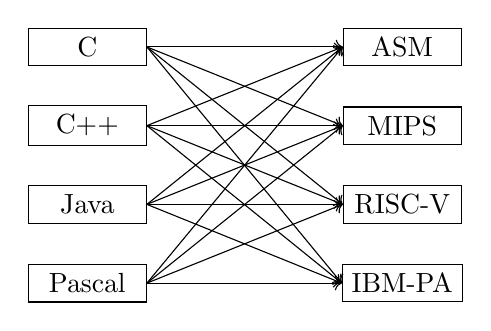
\begin{tikzpicture}
\node (c) [minimum width=1.5cm,draw] at (-2,1.5) {C};
\node (cpp) [minimum width=1.5cm,draw] at (-2,0.5) {C++};
\node (java) [minimum width=1.5cm,draw] at (-2,-0.5) {Java};
\node (pascal) [minimum width=1.5cm,draw] at (-2,-1.5) {Pascal};
\node (asm) [minimum width=1.5cm,draw] at (2,1.5) {ASM};
\node (mips) [minimum width=1.5cm,draw] at (2,0.5) {MIPS};
\node (risc) [minimum width=1.5cm,draw] at (2,-0.5) {RISC-V};
\node (ibm) [minimum width=1.5cm,draw] at (2,-1.5) {IBM-PA};
\draw[->] (c.east) -- (asm.west); \draw[->] (c.east) -- (mips.west);
\draw[->] (c.east) -- (risc.west); \draw[->] (c.east) -- (ibm.west);
\draw[->] (cpp.east) -- (asm.west); \draw[->] (cpp.east) -- (mips.west);
\draw[->] (cpp.east) -- (risc.west); \draw[->] (cpp.east) -- (ibm.west);
\draw[->] (java.east) -- (asm.west); \draw[->] (java.east) -- (mips.west);
\draw[->] (java.east) -- (risc.west); \draw[->] (java.east) -- (ibm.west);
\draw[->] (pascal.east) -- (asm.west); \draw[->] (pascal.east) -- (mips.west);
\draw[->] (pascal.east) -- (risc.west); \draw[->] (pascal.east) -- (ibm.west);
\end{tikzpicture}
\caption{Without Intermediate Language}\label{m-m}
\end{subfigure}
\begin{subfigure}[b]{0.45\textwidth}
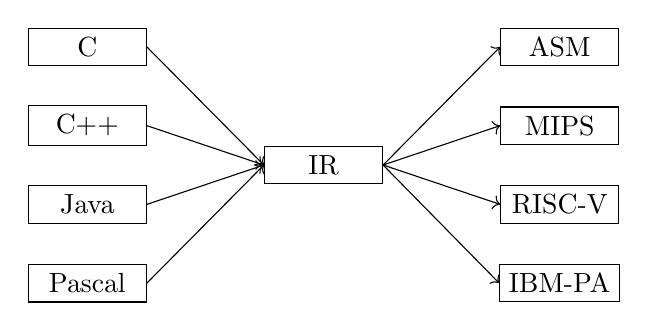
\begin{tikzpicture}
\node (c) [minimum width=1.5cm,draw] at (-3,1.5) {C};
\node (cpp) [minimum width=1.5cm,draw] at (-3,0.5) {C++};
\node (java) [minimum width=1.5cm,draw] at (-3,-0.5) {Java};
\node (pascal) [minimum width=1.5cm,draw] at (-3,-1.5) {Pascal};
\node (asm) [minimum width=1.5cm,draw] at (3,1.5) {ASM};
\node (mips) [minimum width=1.5cm,draw] at (3,0.5) {MIPS};
\node (risc) [minimum width=1.5cm,draw] at (3,-0.5) {RISC-V};
\node (ibm) [minimum width=1.5cm,draw] at (3,-1.5) {IBM-PA};
\node (ir) [minimum width=1.5cm,draw] at (0,0) {IR};
\draw[->] (c.east) -- (ir.west); \draw[->] (cpp.east) -- (ir.west);
\draw[->] (java.east) -- (ir.west); \draw[->] (pascal.east) -- (ir.west);
\draw[->] (ir.east) -- (asm.west); \draw[->] (ir.east) -- (mips.west);
\draw[->] (ir.east) -- (risc.west); \draw[->] (ir.east) -- (ibm.west);
\end{tikzpicture}    
\caption{With Intermediate Language}\label{m-o-m}
\end{subfigure}
\caption{Relationship Between Advanced Programming Languages and Processors, abstracted from textbook \cite{book}}\label{pl-p}
\end{figure}

\section{Dependencies}

\begin{enumerate}
\item JDK version $\geq$ JDK-8. 
\item JavaCC package and MiniJava Parser. 
\item Vapor interpreter.
\end{enumerate}

\section{Methods for Translating}

\subsection{Implementation for V-Table}

We will use V-Table to determine which method to call since method overriding is also allowed in MiniJava. For the details about V-Table, you may refer to the textbook \cite{book}. Here we just provide some details about our implementation. 

Actually we just creat a new class called \texttt{CMPair}. Just like its name says, each instance of \texttt{CMPair} represents a pair of class and method. Note the method may be overriden, so the class will be changed to the subclass instead of superclass. 

We take a sample code segment for example:
\begin{lstlisting}
class A {
	public int run() { ... }
	public int get() { ... }
}

class B extends A {
	public int get() { ... }
}

class C extends B {
	public int run() { ... }
}
\end{lstlisting}

Then the V-Table for them is like
\begin{figure}[H]
\centering
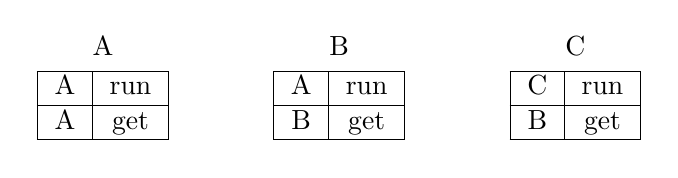
\begin{tikzpicture}
\node at (-3,0) {\begin{tabular}{|c|c|}
\hline A & run \\
\hline A & get \\\hline
\end{tabular}};

\node at (0,0) {\begin{tabular}{|c|c|}
\hline A & run \\
\hline B & get \\\hline
\end{tabular}};

\node at (3,0) {\begin{tabular}{|c|c|}
\hline C & run \\
\hline B & get \\\hline
\end{tabular}};

\node at (-3,0.75) {A}; \node at (0,0.75) {B}; \node at (3,0.75) {C};
\end{tikzpicture}
\caption{V-Table for sample codes}
\end{figure}
where each line represents an instance for \texttt{CMPair}. 

\subsection{Mapping in Scope}

We also notice another problem. Since we will use temporary variable name in intermediate codes, it will be difficult for us to refer to them if we want to use some variables for multiple time. Therefore, for each scope, we will maintain a table recording a mapping from each identifier in java codes to an identifier in vapor code. 

We will also provide an example
\begin{lstlisting}
a = 2;
b = 3;
System.out.println(a + b);
\end{lstlisting}
whose corresponding vapor code will be
\begin{lstlisting}
t.1 = 2
t.2 = 3
t.3 = Add(t.1 t.2)
PrintInt(t.3)
\end{lstlisting}

Then the mapping will be $a\rightarrow t.1$ and $b\rightarrow t.2$. When we want to translate the statement in line 3, we will first find if there exists a record for $a$ and $b$. If we find a matching result, then we will use the allocated identifier in the following translation; otherwise we will create a new identifier for this variable and add this pair to the mapping list. This idea is easy to be implemented and will never occupy so much space. 

Besides, it will reduce the number of identifiers in each scope since we do not need to create a new identifiere

\subsection{Printer Class}

In order to make indent and identifier allocation for vapor, we create a \texttt{Printer} class to deal with it. \texttt{Printer} class contains several methods including:
\begin{enumerate}
\item Record indent number and add indent to the line of the class. 
\begin{lstlisting}
// Add indent to the statement
public void printStmt(String stmt) {
	String statement = "";
	for (int i = 0; i < depth; ++i) {
		statement += "\t";
	}
	statement += stmt;
	System.out.println(statement);
}
\end{lstlisting}
\item Create new identifiers without conflicts. Here we use a counter to generate new identifier. 
\begin{lstlisting}
// Return variable identifier
public String newVariable() {
	String var = "t." + Integer.toString(this.counter);
	incCounter();
	return var;
}
\end{lstlisting}
\item Create label for \texttt{if} and \texttt{while} statements. The idea is similar to the one above. We also set a counter for it. 
\end{enumerate}

\subsection{Dynamic Generation}

During the process of translation, we take a dynamic method instead of a static way. Basically, the ``dynamic'' here means that we generate codes during the visiting process instead output codes after we have traversed the whole code. Actually we do not need to traverse the code again since we have completed symbol table construction and type-checking in last phase. We just need to make use of the symbol table and add V-table and mapping list to the new visitor so that we can directly generate code without refer to other part for the java source code. We provide the generation for some type of expressions. The principle are detailed in homepage \cite{homepage}. 
\begin{lstlisting}
/**
 * f0 -> "while"
 * f1 -> "("
 * f2 -> Expression()
 * f3 -> ")"
 * f4 -> Statement()
 */
public String visit(WhileStatement n) {
	String _ret=null;
	n.f0.accept(this);
	String label = printer.getLCounter();
	printer.printStmt("loop" + label + "_begin:");
	n.f1.accept(this);
	String condition = getStrType(n.f2.accept(this));
	printer.printStmt("if0 " + condition + " goto :loop" + label + "_end");
	n.f3.accept(this);
	printer.incDepth();
	n.f4.accept(this);
	printer.printStmt("goto :loop" + label + "_begin");
	printer.decDepth();
	printer.printStmt("loop" + label + "_end:");
	return _ret;
}

/**
 * f0 -> PrimaryExpression()
 * f1 -> "+"
 * f2 -> PrimaryExpression()
 */
public String visit(PlusExpression n) {
	String _ret=null;
	String left = getStrType(n.f0.accept(this));
	n.f1.accept(this);
	String right = getStrType(n.f2.accept(this));
	_ret = printer.newVariable();
	printer.printStmt(_ret + " = Add(" + left + " " + right + ")");
	return _ret;
}
\end{lstlisting}

\subsection{Some Other Difficulties}

\subsubsection{Fields VS Variables/Parameters}

However, even though we have settled down almost all the problems stated before, we also need to face another two dilemmas. Here is the first one. 

We may encounter some utilizations of a field of class which just look like a normal local variable or parameter. However, though we can allocate a new identifier for the variable and add the mapping to the list of the scope, we cannot apply this method to fields. We need to get the entry address of the instance and add the offset in the class to it. Surprisingly, this is easy since we just need to refer to the record in \texttt{currClass} (For the details of \texttt{currClass}, please refer to the document for phase 1. )
\begin{lstlisting}
private String getStrType(String str) {
	if (this.currClass.findField(str) != null) {	// If it is a field
		int idx = this.currClass.getClassRecord().indexOf(str) * 4 + 4;
		String newVar = printer.newVariable();
		printer.printStmt(newVar + " = [this+" + Integer.toString(idx) + "]");
		return newVar;
	} else if (this.currScope.get(str) != null) {	// If it is an identifier
		return this.currScope.get(str);
	} else {	// It is a value
		return str;
	}
}
\end{lstlisting}

\subsubsection{Variables Not in V-Table}

There is another annoying method call in MiniJava:
\begin{lstlisting}
b = new A().run();
\end{lstlisting}

Yes, we can initially treat it just like what we do for
\begin{lstlisting}
a = new A();
||
t.1 = HeapAllocZ(...)
...
\end{lstlisting}
just return t.1 representing the object, but we cannot add it to the mapping list since there is no matching local varibles or paremeters to it. What a pity! 

If we could find the type of it, then we will be able to determine the offset of the method. Therefore, we need to add a supporting method to determine the class type of it. Since it will be a universal method, then it should also deal with the condition about an instance of a class. We can implement the idea like this:
\begin{lstlisting}
// a method to get type of a class's instance
private String findClassName(PrimaryExpression n) {
	String className = null;
	if (n.f0.choice instanceof AllocationExpression) {	// Class allocation
		AllocationExpression expr = (AllocationExpression)n.f0.choice;
		className = expr.f1.f0.toString();
	} else if (n.f0.choice instanceof ThisExpression) {	// This expression
		className = this.currClass.getName();
	} else if (n.f0.choice instanceof BracketExpression) {
		BracketExpression expr1 = (BracketExpression)n.f0.choice;
		if (expr1.f1.f0.choice instanceof MessageSend) {
			MessageSend expr = (MessageSend)expr1.f1.f0.choice;
			return findClassName(expr.f0);
		}
	} else {	// Parameter / Variable name
		String varName = n.accept(this);
		if (this.currMethod.findParam(varName) != null) {
			className = this.currMethod.findParam(varName).getType();
		} else if (this.currMethod.findVar(varName) != null) {
			className = this.currMethod.findVar(varName).getType();
		} else if (this.currClass.findField(varName) != null) {
			className = this.currClass.findField(varName).getType();
		}
	}
	return className;
}
\end{lstlisting}

\section{Review for Phase 2}

\begin{lstlisting}
==== Results ====
Passed 13/13 test cases
- Submission Size = 67 kB
\end{lstlisting}

Just like phase 1, we also passes all the test cases but I also find something to be improved: how to reduce the number of identifiers we use in vapor code. I checked some outputs of our program and I found some identifiers were never used even though it had been created. That is another optimization problem for us and I am convinced that we can solve it in the future. 

\begin{thebibliography}{9}

\bibitem{homepage}
	Course's Homepage: 
	\href{https://www.cs.ucr.edu/~lesani/teaching/cp/cp.html}{Compiler Project}. 

\bibitem{book}
	Andrew W. Appel, Jens Palsberg, 
	\textit{Modern Compiler Implementation in Java},
	Cambridge University Press, 
	Second Edition, 
	2002. 

\end{thebibliography}

\end{document}
